% chktex-file 1
% !TeX spellcheck = en_GB
% !TeX program = pdflatex
%
% LuxSleek-CV 1.1 LaTeX template
% Author: Andreï V. Kostyrka, University of Luxembourg
%
% 1.1: added tracking and letter-spacing for prettier lower caps, added `~` for language levels
% 1.0: initial release
%
% This template fills the gap in the available variety of templates
% by proposing something that is not a custom class, not using any
% hard-coded settings deeply hidden in style files, and provides
% a handful of custom command definitions that are as transparent as it gets.
% Developed at the University of Luxembourg.
%
% *NOTHING IS HARCODED, and never should be.*
%
% Target audience: applicants in the IT industry, or business in general
%
% The main strength of this template is, it explicitly showcases how
% to break the flow of text to achieve the most flexible right alignment
% of dates for multiple configurations.

\documentclass[11pt, a4paper]{article}

\usepackage[T1]{fontenc}     % We are using pdfLaTeX,
\usepackage[utf8]{inputenc}  % hence this preparation
\usepackage[british]{babel}
\usepackage[left = 0mm, right = 0mm, top = 0mm, bottom = 0mm]{geometry}
\usepackage[stretch = 25, shrink = 25, tracking=true, letterspace=30]{microtype}
\usepackage{graphicx}        % To insert pictures
\usepackage{xcolor}          % To add colour to the document
\usepackage{marvosym}        % Provides icons for the contact details
\usepackage{fontawesome}

\usepackage{enumitem}        % To redefine spacing in lists
\setlist{parsep = 0pt, topsep = 0pt, partopsep = 1pt, itemsep = 1pt, leftmargin = 6mm}

\usepackage{FiraSans}        % Change this to use any font, but keep it simple
\renewcommand{\familydefault}{\sfdefault}

\definecolor{cvblue}{HTML}{304263}

%%%%%%% USER COMMAND DEFINITIONS %%%%%%%%%%%%%%%%%%%%%%%%%%%
% These are the real workhorses of this template
\newcommand{\dates}[1]{\hfill\mbox{\textbf{#1}}} % Bold stuff that doesn’t got broken into lines
\newcommand{\is}{\par\vskip.5ex plus .4ex} % Item spacing
\newcommand{\headleft}[1]{\vspace*{3ex}\textsc{\textbf{#1}}\par%
    \vspace*{-1.5ex}\hrulefill\par\vspace*{0.7ex}}
\newcommand{\headright}[1]{\vspace*{2.5ex}\textsc{\Large\color{cvblue}#1}\par%
     \vspace*{-2ex}{\color{cvblue}\hrulefill}\par}
%%%%%%%%%%%%%%%%%%%%%%%%%%%%%%%%%%%%%%%%%%%%%%%%%%%%%%%%%%%%

\usepackage[colorlinks = true, urlcolor = white, linkcolor = white]{hyperref}

\begin{document}

% Style definitions -- killing the unnecessary space and adding the skips explicitly
\setlength{\topskip}{0pt}
\setlength{\parindent}{0pt}
\setlength{\parskip}{0pt}
\setlength{\fboxsep}{0pt}
\pagestyle{empty}
\raggedbottom

\begin{minipage}[t]{0.28\textwidth} %% Left column -- outer definition
%  Left column -- top dark rectangle
\colorbox{cvblue}{\begin{minipage}[t][5mm][t]{\textwidth}\null\hfill\null\end{minipage}}

\vspace{-.2ex} % Eliminates the small gap
\colorbox{cvblue!90}{\color{white}  %% LEFT BOX
\kern0.09\textwidth\relax% Left margin provided explicitly
\begin{minipage}[t][293mm][t]{0.82\textwidth}
\raggedright
\vspace*{2.5ex}

\Large Alex \textbf{\textsc{Jammes}} \normalsize

% Centering without extra vertical spacing
\null\hfill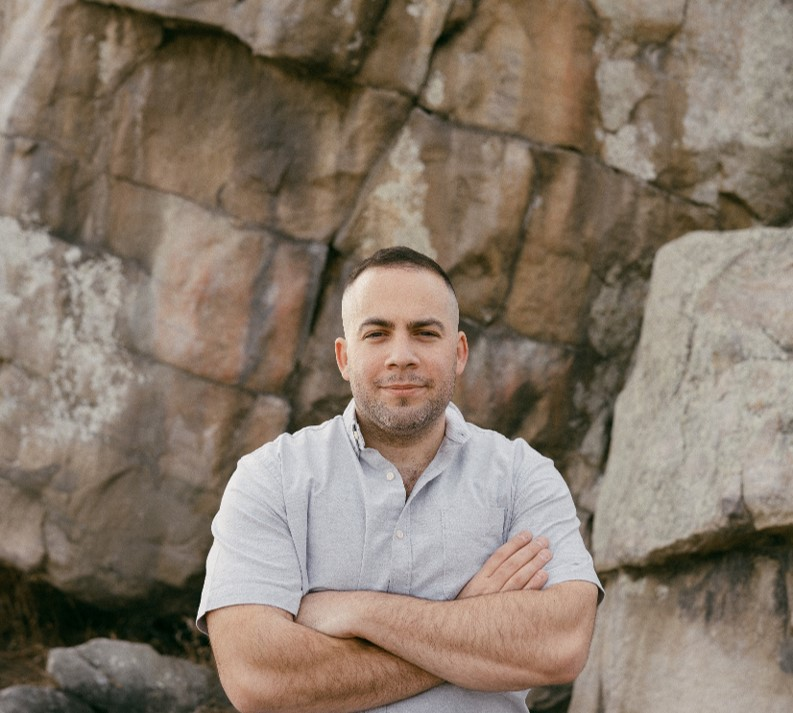
\includegraphics[width=0.65\textwidth]{images/resume_profile_picture.jpg}\hfill\null

\vspace*{0.5ex} % Extra space after the picture

\headleft{Profile Summary}
Dynamic and results-driven individual with over 8+ years of experience in support of \textit{ technical solutions sales} in the Public and Private Cloud space with a proven record of quota achievement. Specializing in Federal verticals with a knack for fostering strong relationships throughout the full sales cycle. Seeking to leverage expertise and skill set to drive sales and build lasting relationships.

\headleft{Contact details}
\small % To fit more content
\MVAt\ {\small ajammes.ftnt@gmail.com} \\[0.4ex]
\faGithub\ {\small github.com/AJLab-GH}\\[0.2ex]
\Mobilefone\ +1\,613\,889\,6564\,\\

\normalsize

\headleft{Personal information}
Citizenship: \textbf{Canadian} \\[0.5ex]
Clearance: \textbf{Secret (2026), Top-Secret Elligibility} \\[0.5ex]
Languages: \textbf{English}, \textbf{French}

\headleft{Skills}
\begin{itemize}
\item Azure, Amazon Web Services, Google Cloud Platform, Oracle Cloud Infrastructure
\item Terraform, AWS CloudFormation, Azure Resource Manager (JSON, BICEP)
\item Docker, Kubernetes, AKS, EKS
\item Azure Pipelines, AWS Code Pipeline, Azure DevOps, Jenkins
\item GitHub, Devcontainers, SAST, DAST, SBOM, SCA
\end{itemize}

\end{minipage}%
\kern0.09\textwidth\relax%%Right margin provided explicitly to stretch the colourbox
}
\end{minipage}% Right column
\hskip2.5em% Left margin for the white area
\begin{minipage}[t]{0.61\textwidth}
\setlength{\parskip}{0.8ex}% Adds spaces between paragraphs; use \\ to add new lines without this space. Shrink this amount to fit more data vertically

\vspace{2ex}

\headright{Experience}

\textsc{Consulting System Engineer --- Cloud Architect} at \textit{Fortinet (Canada).}  \dates{2022.04--Present} \\

\small{Strategic Sales Support --- Served as a pivotal technical resource for strategic pre-sales engagements across
Canada, closely working with Fortinet Sales representatives to design and recommend security solutions that best
meet specific customer needs, ensuring quality and satisfaction.}

\is
\small{Customer and Partner Engagements --- Conducted high-impact technical meetings, presentations, and product
demonstrations for both customers and channel partners, showcasing Fortinet's product strengths and capabilities.}

\is
\small{Solution Architecture and Design --- Collaborated with SE peers in leading the design and architecture of secure IP
networks, leveraging all facets of Fortinet's product line, ensuring the delivery of superior solutions even in
competitive scenarios.}

\is
\small{Technical Consultancy --- Acted as the subject-matter expert in pre-sales design reviews, providing technical
guidance, leadership, and consultation to Field Systems Engineers to shape positive customer outcomes.}

\is
\small{Training \& Mentorship --- Spearheaded training sessions for System Engineers nation-wide and provided
mentorship to SE specialists within Virtual Teams, enhancing their technical capabilities.}

\is
\small{Cross-functional Collaboration --- Worked in tandem with the Engineering team to identify, qualify, and contribute
to the development of critical features that reinforce Fortinet's market position.}

\is
\small{Technical Documentation --- Crafted comprehensive technical documents and guides to improve and expedite
product demonstrations, highlighting Fortinet's product advantages.}

\vspace{2ex}
\textsc{Presales Security Expert --- Cloud Architect} at \textit{Fortinet  (Federal).} \dates{2019.06--2022.04}\\

\small{Sales calls --- main technical resource on sales calls and answer/ educate the customer on issues ranging from
features, specifications and functionality to integration. Conversant with networking applications and solutions.}

\is
\small{Selling --- Successfully sold solutions tailored to the Federal vertical, reinforcing company presence in the
Federal sector.}

\is
\small{Significant deal size --- Closed multiple high-value deals, resulting in significant revenue growth for the company.
Presentations --- Delivered compelling presentations to both C-suite executives and individual team members,
ensuring buy-in at all organizational levels.}

\vspace{2ex}
\textsc{Diamond Services Engineer \& TAC} at \textit{Check Point (North America).} \dates{2017.01--2019.06}\\

\small{Customer Engagement — Played a key role in the design, deployment, and maintenance of cloud security solutions for Fortune 100 companies. Additionally, led training on public and private cloud solutions for both internal stakeholders and customers across Canada, the United States, and internationally.}

\headright{Education}

\textsc{Network Security Professional Program.} \textit{from Willis College}. \dates{2015--2016} \\

\headright{Fun Facts}

\textit{This resume was created and delivered as Code.}

\end{minipage}

\end{document}
